\documentclass[dvips,12pt]{article}

\usepackage[pdftex]{graphicx}
\usepackage{subcaption}
\usepackage{float}
\usepackage{url}
\usepackage[utf8]{inputenc}
\usepackage{geometry}
\usepackage{setspace}
\usepackage{amsmath}
\usepackage{txfonts}

% From amsmath, prepend equation numbers with section number
%\numberwithin{equation}{section}

% graphicx: Where should graphics be found?
\graphicspath{ {figures/} }

% Setup margins and paper size
\geometry{
  letterpaper,
  total={170mm,257mm},
  left=20mm,
  top=20mm,
  bottom=25mm
}

\makeatletter % changes the catcode of @ to 11
\renewcommand*\env@matrix[1][*\c@MaxMatrixCols c]{%
  \hskip -\arraycolsep
  \let\@ifnextchar\new@ifnextchar
  \array{#1}}
\makeatother % changes the catcode of @ back to 12

% -----------------------------------------------------------------------------

\begin{document}

% Article Title
\title{\LARGE The Desktop Quad }
\author{Parker Lusk}
\date{\today}
\maketitle

\begin{abstract}
	The Desktop Quad is an effort to allow an inexpensive quadrotor to be used as a case study in controls, vision processing, and autopilot design scenarios. It features an 8cm x 8cm quadrotor with an upward-facing camera for localization. The (really) micro air vehicle (MAV) is tethered using silicone wire for communications and power, allowing indefinite flight. This report describes the progress of the Desktop Quad achieving fully autonomous flight.
\end{abstract}

\doublespacing
% -----------------------------------------------------------------------------
\section{Introduction}

% -----------------------------------------------------------------------------
\section{Hardware Selection}

% -----------------------------------------------------------------------------
\section{Flight Controller}

% -----------------------------------------------------------------------------
\section{Building the System}

% -----------------------------------------------------------------------------
\section{Visual Localization}

% -----------------------------------------------------------------------------
\section{Simulation}

% -----------------------------------------------------------------------------
\section{Control Architecture}

\begin{figure}[H]
	\centering
	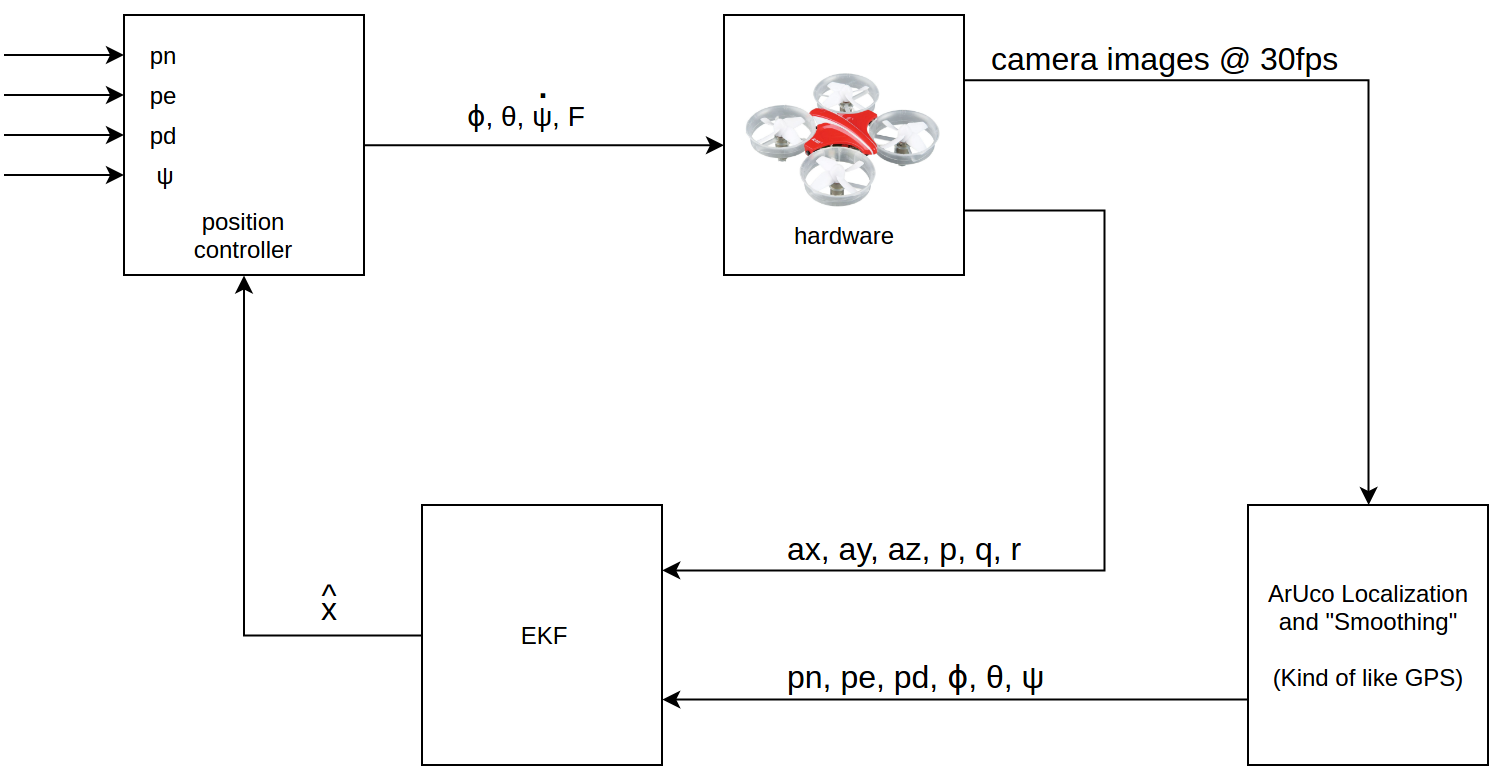
\includegraphics[width=\textwidth]{desktopquad_control_arch}
	\caption{Control architecture of the Desktop Quad system.}
	\label{fig:architecture}
\end{figure}


\begin{thebibliography}{9}
\singlespace

\bibitem{UAVBook} R. W. Beard and T. W. McLain, “Small unmanned aircraft,” 2011.

\bibitem{Beard2016} R. W. Beard and T. W. Mclain, “Introduction to Feedback Control using Design Studies,” 2016.

\bibitem{Ferrin2011} J. Ferrin, R. Leishman, R. Beard, and T. McLain, “Differential flatness based control of a rotorcraft for aggressive maneuvers,” IEEE Int. Conf. Intell. Robot. Syst., pp. 2688–2693, 2011.

\bibitem{Albasiouny2016} E. R. Albasiouny, A. Sarhan, and T. Medhat, “Mean-shift-FAST algorithm to handle motion-blur with tracking fiducial markers,” Proc. - 2015 10th Int. Conf. Comput. Eng. Syst. ICCES 2015, no. December, pp. 286–292, 2016.

\bibitem{aruco2014} S. Garrido-Jurado, R. Muñoz-Salinas, F. J. Madrid-Cuevas, and M. J. Marín-Jiménez, “Automatic generation and detection of highly reliable fiducial markers under occlusion,” Pattern Recognit., vol. 47, no. 6, pp. 2280–2292, 2014.

\bibitem{apriltag2011} E. Olson, “AprilTag: A robust and flexible visual fiducial system,” Proc. - IEEE Int. Conf. Robot. Autom., pp. 3400–3407, 2011.

\bibitem{Prasad2015} M. G. Prasad, S. Chandran, and M. S. Brown, “A motion blur resilient fiducial for quadcopter imaging,” Proc. - 2015 IEEE Winter Conf. Appl. Comput. Vision, WACV 2015, pp. 254–261, 2015.

\end{thebibliography}

\end{document}